\documentclass[12pt]{article}
\usepackage[utf8]{inputenc}
\usepackage[slovene]{babel}

\usepackage{hyperref}
\usepackage{listings} % za naslovnico
\usepackage{amsthm}
\usepackage{amsmath, amssymb, amsfonts}
\usepackage{graphicx}


%\graphicspath{ {./Slike/} }
\usepackage{subcaption} % za side-by-side slike
\usepackage[
top    = 2.cm,
bottom = 2.cm,
left   = 2.cm,
right  = 2.cm]{geometry}

\usepackage{footnote}
\makesavenoteenv{tabular}
\title{Domača naloga - 1.del \\
\large Izbira metode in optimizacija hiperparametrov}

\begin{document}
    
\author{Vito Rozman}
\date{\today}
\maketitle



\section{Izbira in evalvacija modelov}

Za ročno iskanje najboljšega modela sem izbral \emph{knn}, \emph{svm} in \emph{rf}. 
Podatke sem najprej razdelil v razmerju 1:4 na testne in učne. Na učnih sem preverjal 
točnost modela z AUC metriko (ploščino pod ROC krvuljo) z metodo prečnega preverjanja 
(ang. cross validation).
Potem sem testeral model še na testnih podatkih. Iskal sem model z naboljšim rezultatom AUC 
\emph{cross validation}.
Opisan potopek sem najprej izvedel na neskaliranih podatkih, potem pa še na skaliranih, 
ter primerjal
rezultate. Iskazalo se je da so skalirani podatki bolje obnesli, vendar pri izbiri 
najboljšega modela niso privedli do večjih razlik.
\subsection{Hiperparamatri pri ročnem iskanju}
\textbf{Najbližji sosede:} parameter $k=1:30$\\
\textbf{Podporni vektorji:} izbira 
\emph{jedra} $\in \{\text{linearno}, \text{polinomsko}, \text{sigmoidno}\}$, 
parametr $C=\{1, 10\}$\\
\textbf{Naključni gozdovi:} parameter \emph{največja dovoljena globina} $\in \{2, 7, 12, 17, 22, 27, 32, 37, 42, 47\}$,
parameter \emph{najmaša radelitev vzorca} $\in \{1, 3, 5, 7, 9, 11, 13, 15, 17, 19\}$
\subsection{Hiperparamatri pri avtomatiziranem iskanju}
Pri avtomatiziranem iskanje pa sem izbral enake hiperparametre kot pri ročnem, razen pri naključnih gozdovih 
sem dodal parameter \emph{minimalno število primerov v listu}$\in \{1, 2, 3\}$.

\section{Zmogljivosti algoritmov}

Z izbiro hiperparametrev pri obeh prezkusih sem želel testirati kako učinkovito je avtomatizirano
iskanje najbolšega modela in sem predvideval, da bom pri obeh dobil ista modela. Za izbiro
parametov pa sem bil malo presenečen, da nisem dobil tako podobnih rezultatov. Pri rf na 
sliki \ref{fig:rf1} in sliki \ref{fig:rf2} vidimo, da za majhno vrednost max-depth dobimo 
slab rezultat, v vseh ostalik kofiguracijah pa so rezultati primerljivo podobni. Morda 
bi bilo smiselno vzeti več paramatrov z večjim korakom. Na sliki \ref{fig:knn} vidimo, da večanje 
število sosedov izbolšuje AUC modela. Zaradi malega števila različnih parametrov je na sliki 
\ref{fig:svm} vidno, da so različne konfiguracije z večimi poizkušanji privedle podobne
rezultate.


\begin{figure}[!htb]
    \minipage{0.45\textwidth}
      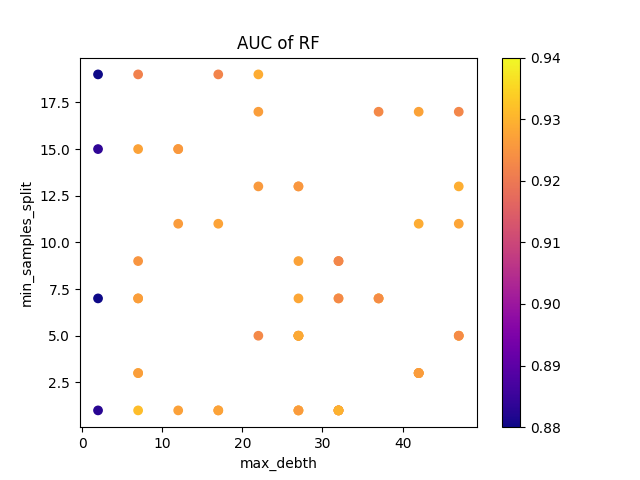
\includegraphics[width=\linewidth]{fig/rf1.png}
      \caption{Zmogljivost \emph{rf} glede na parametra max-depth in min-sample-split}
      \label{fig:rf1}
    \endminipage\hfill
    \minipage{0.45\textwidth}
      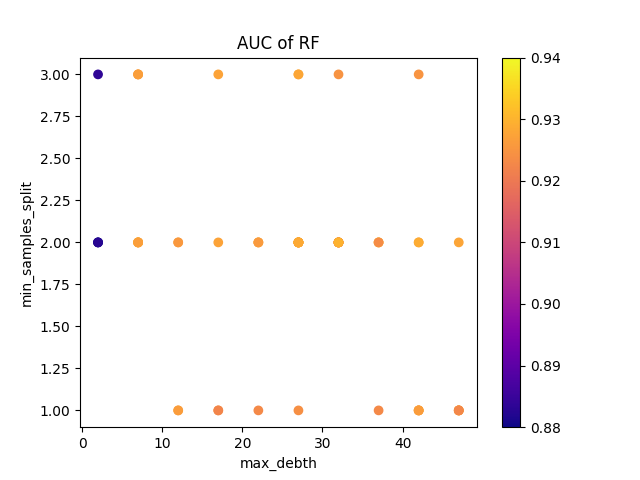
\includegraphics[width=\linewidth]{fig/rf2.png}
      \caption{Zmogljivost \emph{rf} glede na parametra max-depth in min-sample-leaf}
      \label{fig:rf2}
    \endminipage
\end{figure}

\begin{figure}[!htb]
    \minipage{0.45\textwidth}
      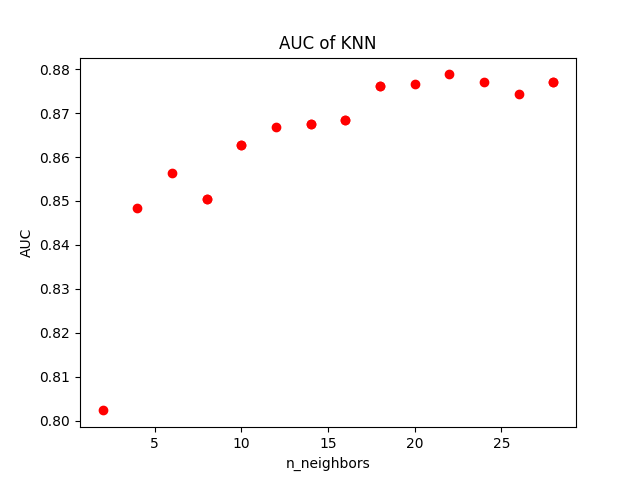
\includegraphics[width=\linewidth]{fig/knn.png}
      \caption{Zmogljivost \emph{knn} glede na parameter n-neighbors}
      \label{fig:knn}
    \endminipage\hfill
    \minipage{0.45\textwidth}
      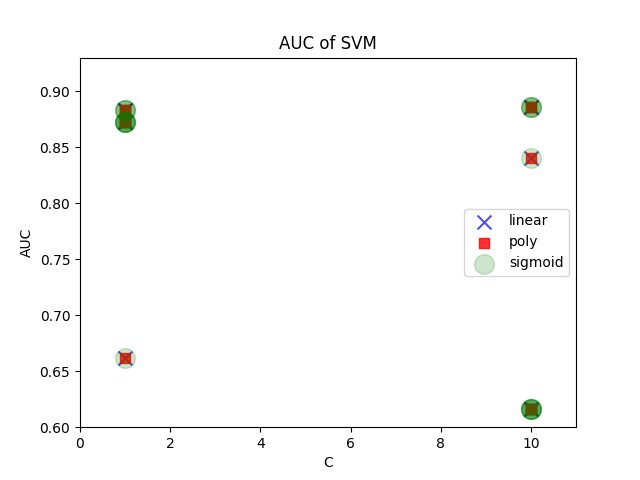
\includegraphics[width=\linewidth]{fig/svm.png}
      \caption{Zmogljivost \emph{svm} glede na jerdo in parameter C}
      \label{fig:svm}
    \endminipage
\end{figure}


\subsection{Najboljši model in njegovi hiperparametri}
\textbf{Ročno iskanje} Najbolje se je izkazal model \emph{rf} z izbranimi prarametri: 
\emph{max-depth}$=37$ in \emph{min-sample-split}$=3$.\\
\textbf{Avtomatizirano iskanje} Najbolje se je izkazal model \emph{rf} z izbranimi prarametri: 
\emph{max-depth}$=27$, \emph{min-sample-split}$=1$ in \emph{min-sample-leaf}$=2$.
\begin{center}
    \begin{tabular}{||c| c c||} 
        \hline
        \emph{rf}  & AUC - cross validation &  AUC test set  \\ [0.5ex] 
        \hline\hline
        Ročno & 0.928039  & 0.887989 \\
        \hline
        Avtomatizirano & 0.928101 & 0.847335\\
        \hline
    \end{tabular}
\end{center}


\section{Zaključek}

Avtomatizirano iskanje najboljšega modela in njegovih hiperparametriv se je izkazalo za 
dokaj učinkovi pristop, saj sem dobil podobne rezultate pri kot pri ročnem iskanju. 
Zanimivo mi je bilo, da ko sem uporabil skalirane podatke je \emph{hiperopt} deloval veliko 
hiteje kot z neskaliranimi podatki.

\end{document}